\everymath{\displaystyle}
\documentclass{beamer}
% \documentclass[handout]{beamer}

%\usepackage[pdftex]{color,graphicx}
\usepackage{amsmath,amssymb,amsfonts}

\mode<presentation>
{
  % \usetheme{Darmstadt}
  % \usetheme[hideothersubsections]{Hannover}
  % \usetheme[hideothersubsections]{Goettingen}
  \usetheme[hideothersubsections, right]{Berkeley}

  \usecolortheme{seahorse}
  % \usecolortheme{dolphin}
  \usecolortheme{rose}
  % \usecolortheme{orchid}

  \useinnertheme[shadow]{rounded}

  \setbeamercovered{transparent}
  % or whatever (possibly just delete it)
}

\mode<handout>{
  \setbeamercolor{background canvas}{bg=black!5}
  \usepackage{pgfpages}
  \pgfpagesuselayout{4 on 1}[a4paper,border shrink=5mm, landscape]
}

\usepackage[brazilian]{babel}
% or whatever

% \usepackage[latin1]{inputenc}
\usepackage[utf8]{inputenc}
% or whatever

\usepackage{times}
%\usepackage[T1]{fontenc}
% Or whatever. Note that the encoding and the font should match. If T1
% does not look nice, try deleting the line with the fontenc.

% \usepackage[T1]{fontenc}
% \usepackage{lmodern}

\title%[] % (optional, use only with long paper titles)
{Bioestatística}

\subtitle
{Análise de Dados} % (optional)

\author%[] % (optional, use only with lots of authors)
{Felipe Figueiredo}% \and S.~Another\inst{2}}
% - Use the \inst{?} command only if the authors have different
%   affiliation.

\institute[INTO] % (optional, but mostly needed)
{Instituto Nacional de Traumatologia e Ortopedia
}
  % \inst{1}%
  % Department of Computer Science\\
  % University of Somewhere
  % \and
  % \inst{2}%
  % Department of Theoretical Philosophy\\
  % University of Elsewhere}
% - Use the \inst command only if there are several affiliations.
% - Keep it simple, no one is interested in your street address.

\date%[] % (optional)
{}

% \subject{Talks}
% This is only inserted into the PDF information catalog. Can be left
% out. 



% If you have a file called "university-logo-filename.xxx", where xxx
% is a graphic format that can be processed by latex or pdflatex,
% resp., then you can add a logo as follows:

\pgfdeclareimage[height=1.6cm]{university-logo}{../logo}
\logo{\pgfuseimage{university-logo}}



% Delete this, if you do not want the table of contents to pop up at
% the beginning of each subsection:
\AtBeginSubsection[]
%\AtBeginSection[]
{
  \begin{frame}<beamer>{Sumário}
    \tableofcontents[currentsection,currentsubsection]
  \end{frame}
}


% If you wish to uncover everything in a step-wise fashion, uncomment
% the following command: 

% \beamerdefaultoverlayspecification{<+->}


\begin{document}

\begin{frame}
  \titlepage
\end{frame}

\begin{frame}{Sumário}
  \tableofcontents
  % You might wish to add the option [pausesections]
\end{frame}


%% Template
% \section{}

% \subsection{}

% \begin{frame}{}
%   \begin{itemize}
%   \item 
%   \end{itemize}
% \end{frame}

% \begin{frame}
%   \begin{columns}
%     \begin{column}{5cm}
%     \end{column}
%     \begin{column}{5cm}
%     \end{column}
%   \end{columns}
% \end{frame}

% \begin{frame}{}
%   \includegraphics[height=0.4\textheight]{file1}
%   \includegraphics[height=0.4\textheight]{file2}
%   \includegraphics[height=0.4\textheight]{file3}
%   \begin{figure}
%     \caption{}
%   \end{figure}
% \end{frame}

% \begin{frame}{}
%   \begin{definition}
%   \end{definition}
%   \begin{example}
%   \end{example}
%   \begin{block}{Exercício}
%   \end{block}
% \end{frame}


\section{Apresentação}

\subsection{O docente e material online}

\begin{frame}{Docente}
  \begin{block}{Nome}
    Felipe Figueiredo
  \end{block}
  \begin{block}{Email}
    \url{prof.felipefigueiredo@gmail.com}

    \bigskip
    \small
    \alert{Atenção:} Salve-o como contato e use o endereço salvo, para mitigar a chance de {\bf estravio}!
    \footnote{O endereço felipefigueiredo@gmail.com {\bf não é meu}!}
  \end{block}
\end{frame}

\begin{frame}{Material online}
  Todo o material didático será disponibilizado na página da disciplina, que fica no Site abaixo
  \begin{block}{Site (http / https)}
    \small
    \url{sites.google.com/site/proffelipefigueiredo/}
  \end{block}
  % Adicionalmente, avisos importantes podem ser divulgados no blog
  % \begin{block}{Blog}
  %   \small
  %   \url{http://proffelipefigueiredo.blogspot.com.br/}
  % \end{block}

  \bigskip
  O endereço não é de fácil memorização, portanto uma busca no Google é o melhor caminho.

  \bigskip
  Você pode procurar pelo meu nome (Felipe Figueiredo)

  \bigskip
  \bigskip
  Porém...
\end{frame}

\begin{frame}{Google: felipe figueiredo}
  \begin{center}
    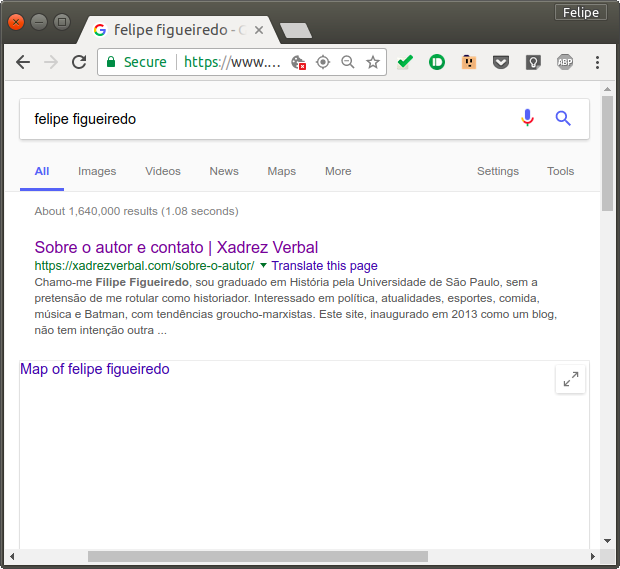
\includegraphics[height=.7\textheight]{Intro/felipefigueiredo-not1}
    \begin{exampleblock}{}
      \begin{center}
        {\bf Não sou Historiador}
      \end{center}
    \end{exampleblock}
  \end{center}
\end{frame}

\begin{frame}{Google: dr felipe figueiredo}
  \begin{center}
    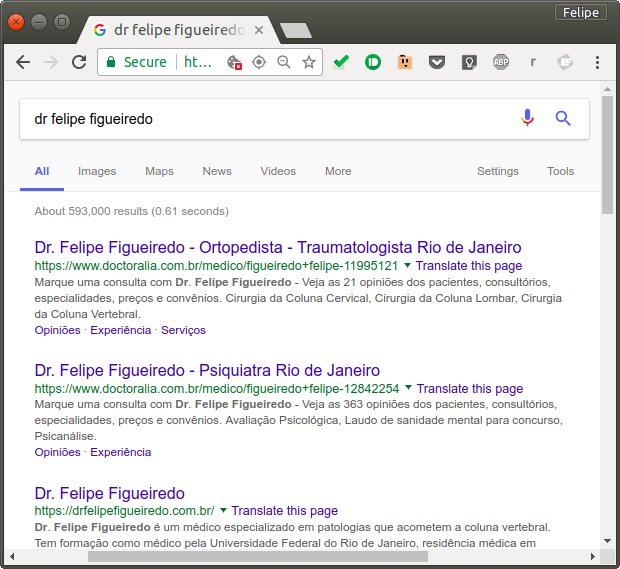
\includegraphics[height=.7\textheight]{Intro/felipefigueiredo-not2}
    \begin{exampleblock}{}
      \begin{center}
        {\bf Não sou Psiquatra ou Ortopedista}
      \end{center}
    \end{exampleblock}
  \end{center}
\end{frame}

\begin{frame}{Google: prof felipe figueiredo}
  \begin{center}
    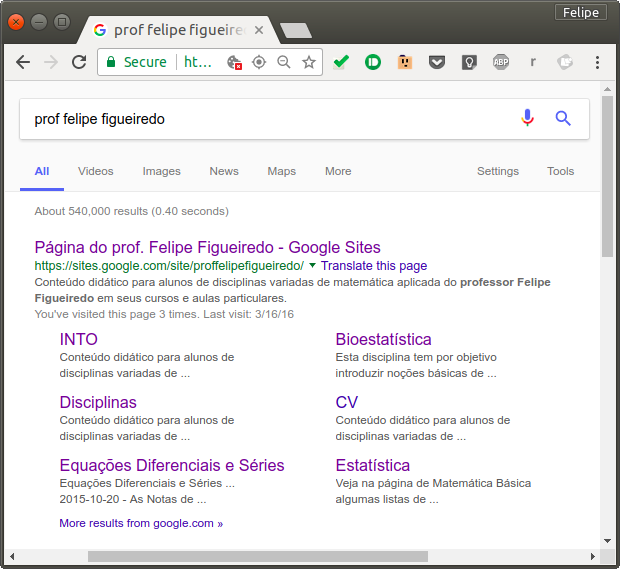
\includegraphics[height=.7\textheight]{Intro/felipefigueiredo}
    \begin{exampleblock}{}
      \begin{center}
        Este que vos fala, a seu dispor.
      \end{center}
    \end{exampleblock}
  \end{center}
\end{frame}

\begin{frame}{Material online}
  \begin{center}
    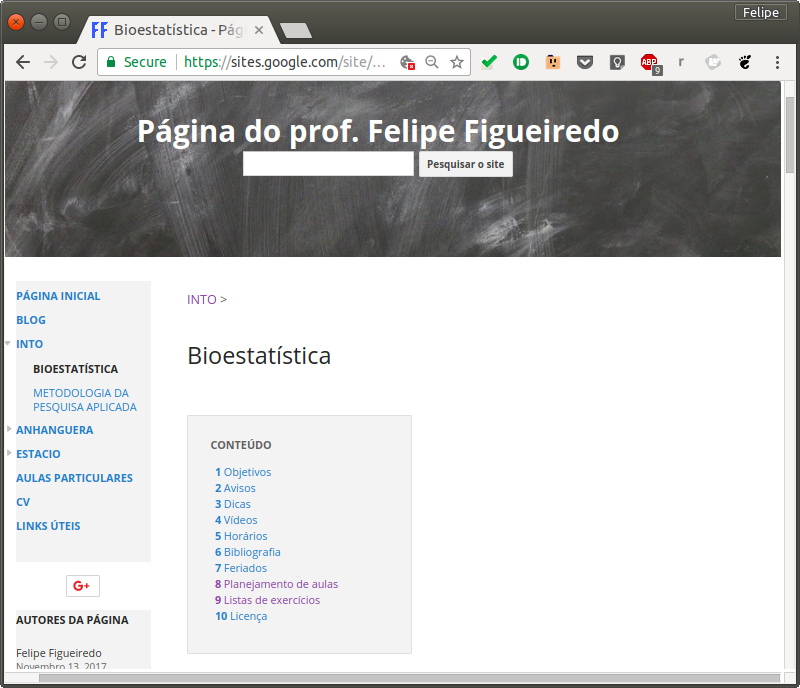
\includegraphics[height=.7\textheight]{Intro/pg-disciplina}
    \begin{exampleblock}{}
      \begin{center}
        PDFs das aulas, artigos, livros, vídeos, exercícios...
      \end{center}
    \end{exampleblock}
  \end{center}
\end{frame}

\subsection{A disciplina}

\begin{frame}{Objetivos de aprendizagem}
  \begin{block}{}
    Interpretar criticamente dados e resultados de artigos científicos.
  \end{block}
\end{frame}

\begin{frame}{Aprendizado pós-aula}
  \begin{block}{Leitura}
    \begin{itemize}
    \item Listas de leitura obrigatória, e a leitura recomendada
    \item É fundamental ler as seções obrigatórias
    \item As aulas seguintes presumem esta leitura
    \item Tire suas dúvidas ({\small presencial, e-mail, pombo-correio...})
    \item É fundamental ler as seções obrigatórias
    \end{itemize}
  \end{block}
  \begin{block}{Listas de exercícios}
    \begin{itemize}
    \item Breve lista de exercícios de fixação
    \item Em geral, questões de interpretação de resultados
    \item Entrega em datas programadas
    \end{itemize}
  \end{block}
\end{frame}

\begin{frame}{Bibliografia}
  \begin{block}{Livro texto}
    Motulsky, Harvey J. (1995) {\em Intuitive Biostatistics}, 1st ed - Oxford Press
  \end{block}
  \begin{itemize}
  \item Alguns capítulos (3a edição) disponíveis gratuitamente no site da editora\footnote{links na página da disciplina}
  \item Fontes de apoio online (apostilas e papers).
  \end{itemize}
\end{frame}

\subsection{Avaliação}

\begin{frame}{Avaliação}
  \begin{itemize}
  \item {\bf Objetivo:} interpretar criticamente um paper
  \item Seminário (grupo)
  \item Dois últimos encontros
  \item Roteiro disponível para auxiliar a elaboração.
  \end{itemize}
\end{frame}

\section{Bioestatística}

\begin{frame}{O que é}
  \begin{columns}
    \begin{column}{7cm}
      \begin{block}{}
        {\scriptsize ``{\em The Statistician is the Wizard who makes
            `scientific' statements about invisible states and
            quantities. However, contrary to the real wishes (or
            witches), he attaches uncertainties to his statements}'' –
          Carlos A.  Pereira.}
      \end{block}
      \begin{block}{}
        {\scriptsize ``{\em Se você torturar os dados o suficiente,
            eles confessarão o que você quiser.}'' - Ronald H. Coase}
      \end{block}

    \end{column}
    \begin{column}{3cm}
      \begin{center}
        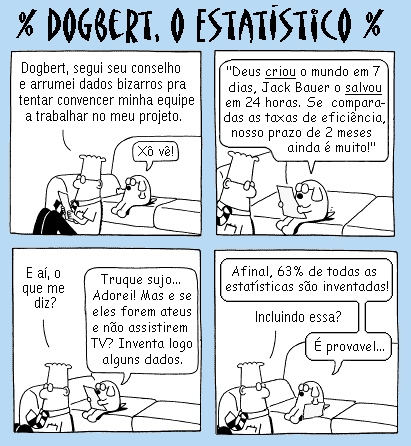
\includegraphics[width=1.6\textwidth]{Intro/dilbert}
      \end{center}
    \end{column}
  \end{columns}
\end{frame}

\begin{frame}{Método Científico}
  \begin{enumerate}
  \item Observação do fenômeno (problema)
  \item Formulação de uma hipótese
  \item Experimento
  \item Validação ou refutação da hipótese
  \end{enumerate}
\end{frame}

\begin{frame}{Método Científico}
  \begin{itemize}
  \item Experimentos tem incertezas
    \begin{itemize}
    \item Coleta de dados imperfeita
    \item Incompletude dos dados
    \item Erros de medição
    \item Formulação incompleta de hipóteses
    \end{itemize}

  \end{itemize}
\end{frame}

\begin{frame}{Método Estatístico}
  \begin{itemize}
  \item Como extrair informação a partir dos dados?
  \item Como lidar com as incertezas?
  \end{itemize}

  \begin{center}
    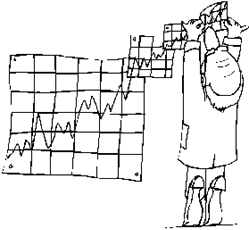
\includegraphics[height=.4\textheight]{Intro/Probabilidades}
  \end{center}
\end{frame}

% \begin{frame}{Método Estatístico}
%   \begin{enumerate}
%   \item Planejamento do experimento
%   \item Coleta/aquisição dos dados
%   \item Organização e descrição dos dados
%   \item Análise/interpretação
%   \item Informação/tomada de decisão
%   \end{enumerate}
% \end{frame}

\begin{frame}{Áreas da Estatística}
  \begin{itemize}
  \item Análise Descritiva
  \item Probabilidade
  \item Inferência
  \item Modelagem
  \end{itemize}
\end{frame}

\begin{frame}{Para que serve}
  \begin{itemize}
  \item Estimação estatística
  \item Teste de hipótese estatístico
  \item Modelagem estatística
  \end{itemize}
\end{frame}

% \section{Trailer do curso}

% \begin{frame}{Dados}
%   \begin{itemize}
%   \item Qualitativos (contagens/proporções)
%   \item Quantitativos (medidas/mensurações)
%   \end{itemize}
% \end{frame}

\begin{frame}{Tipos de Dados}
Dados podem ser classificadas em duas principais categorias
  \begin{itemize}
  \item Qualitativos (categóricos)
  \item Quantitativos (numéricos)
  \end{itemize}
  \begin{example}
    Pressão sistólica (mmHg), altura (cm), sexo (M ou F), grau de
    satisfação com atendimento médico (escore de 1 a 5), perímetro
    abdominal (cm), contagem de leucócitos, número de pessoas na
    família, cor da pele (branco, negro, pardo), etc.
  \end{example}

\end{frame}

% \begin{frame}{Descrição dos Dados}
%   \begin{itemize}
%   \item Organização/visualização
%     \begin{itemize}
%     \item Tabelas
%     \item Gráficos
%     \end{itemize}
%   \item Medidas sumárias
%     \begin{itemize}
%     \item Medidas de tendência central
%     \item Medidas de dispersão
%     \end{itemize}
%   \end{itemize}
% \end{frame}

% \begin{frame}{Trailer do curso}
%   \begin{columns}
%     \begin{column}{5cm}
%       \begin{center}
%         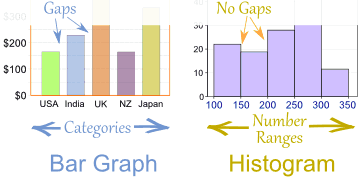
\includegraphics[width=.9\textwidth]{Intro/bar-chart-vs-histogram}

%       \bigskip
%       \bigskip
%       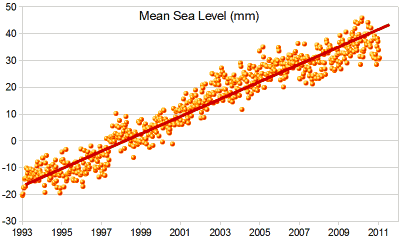
\includegraphics[width=.9\textwidth]{Intro/mean-sea-level-line}
%       \end{center}
%     \end{column}
%     \begin{column}{6cm}
%       \begin{center}
%         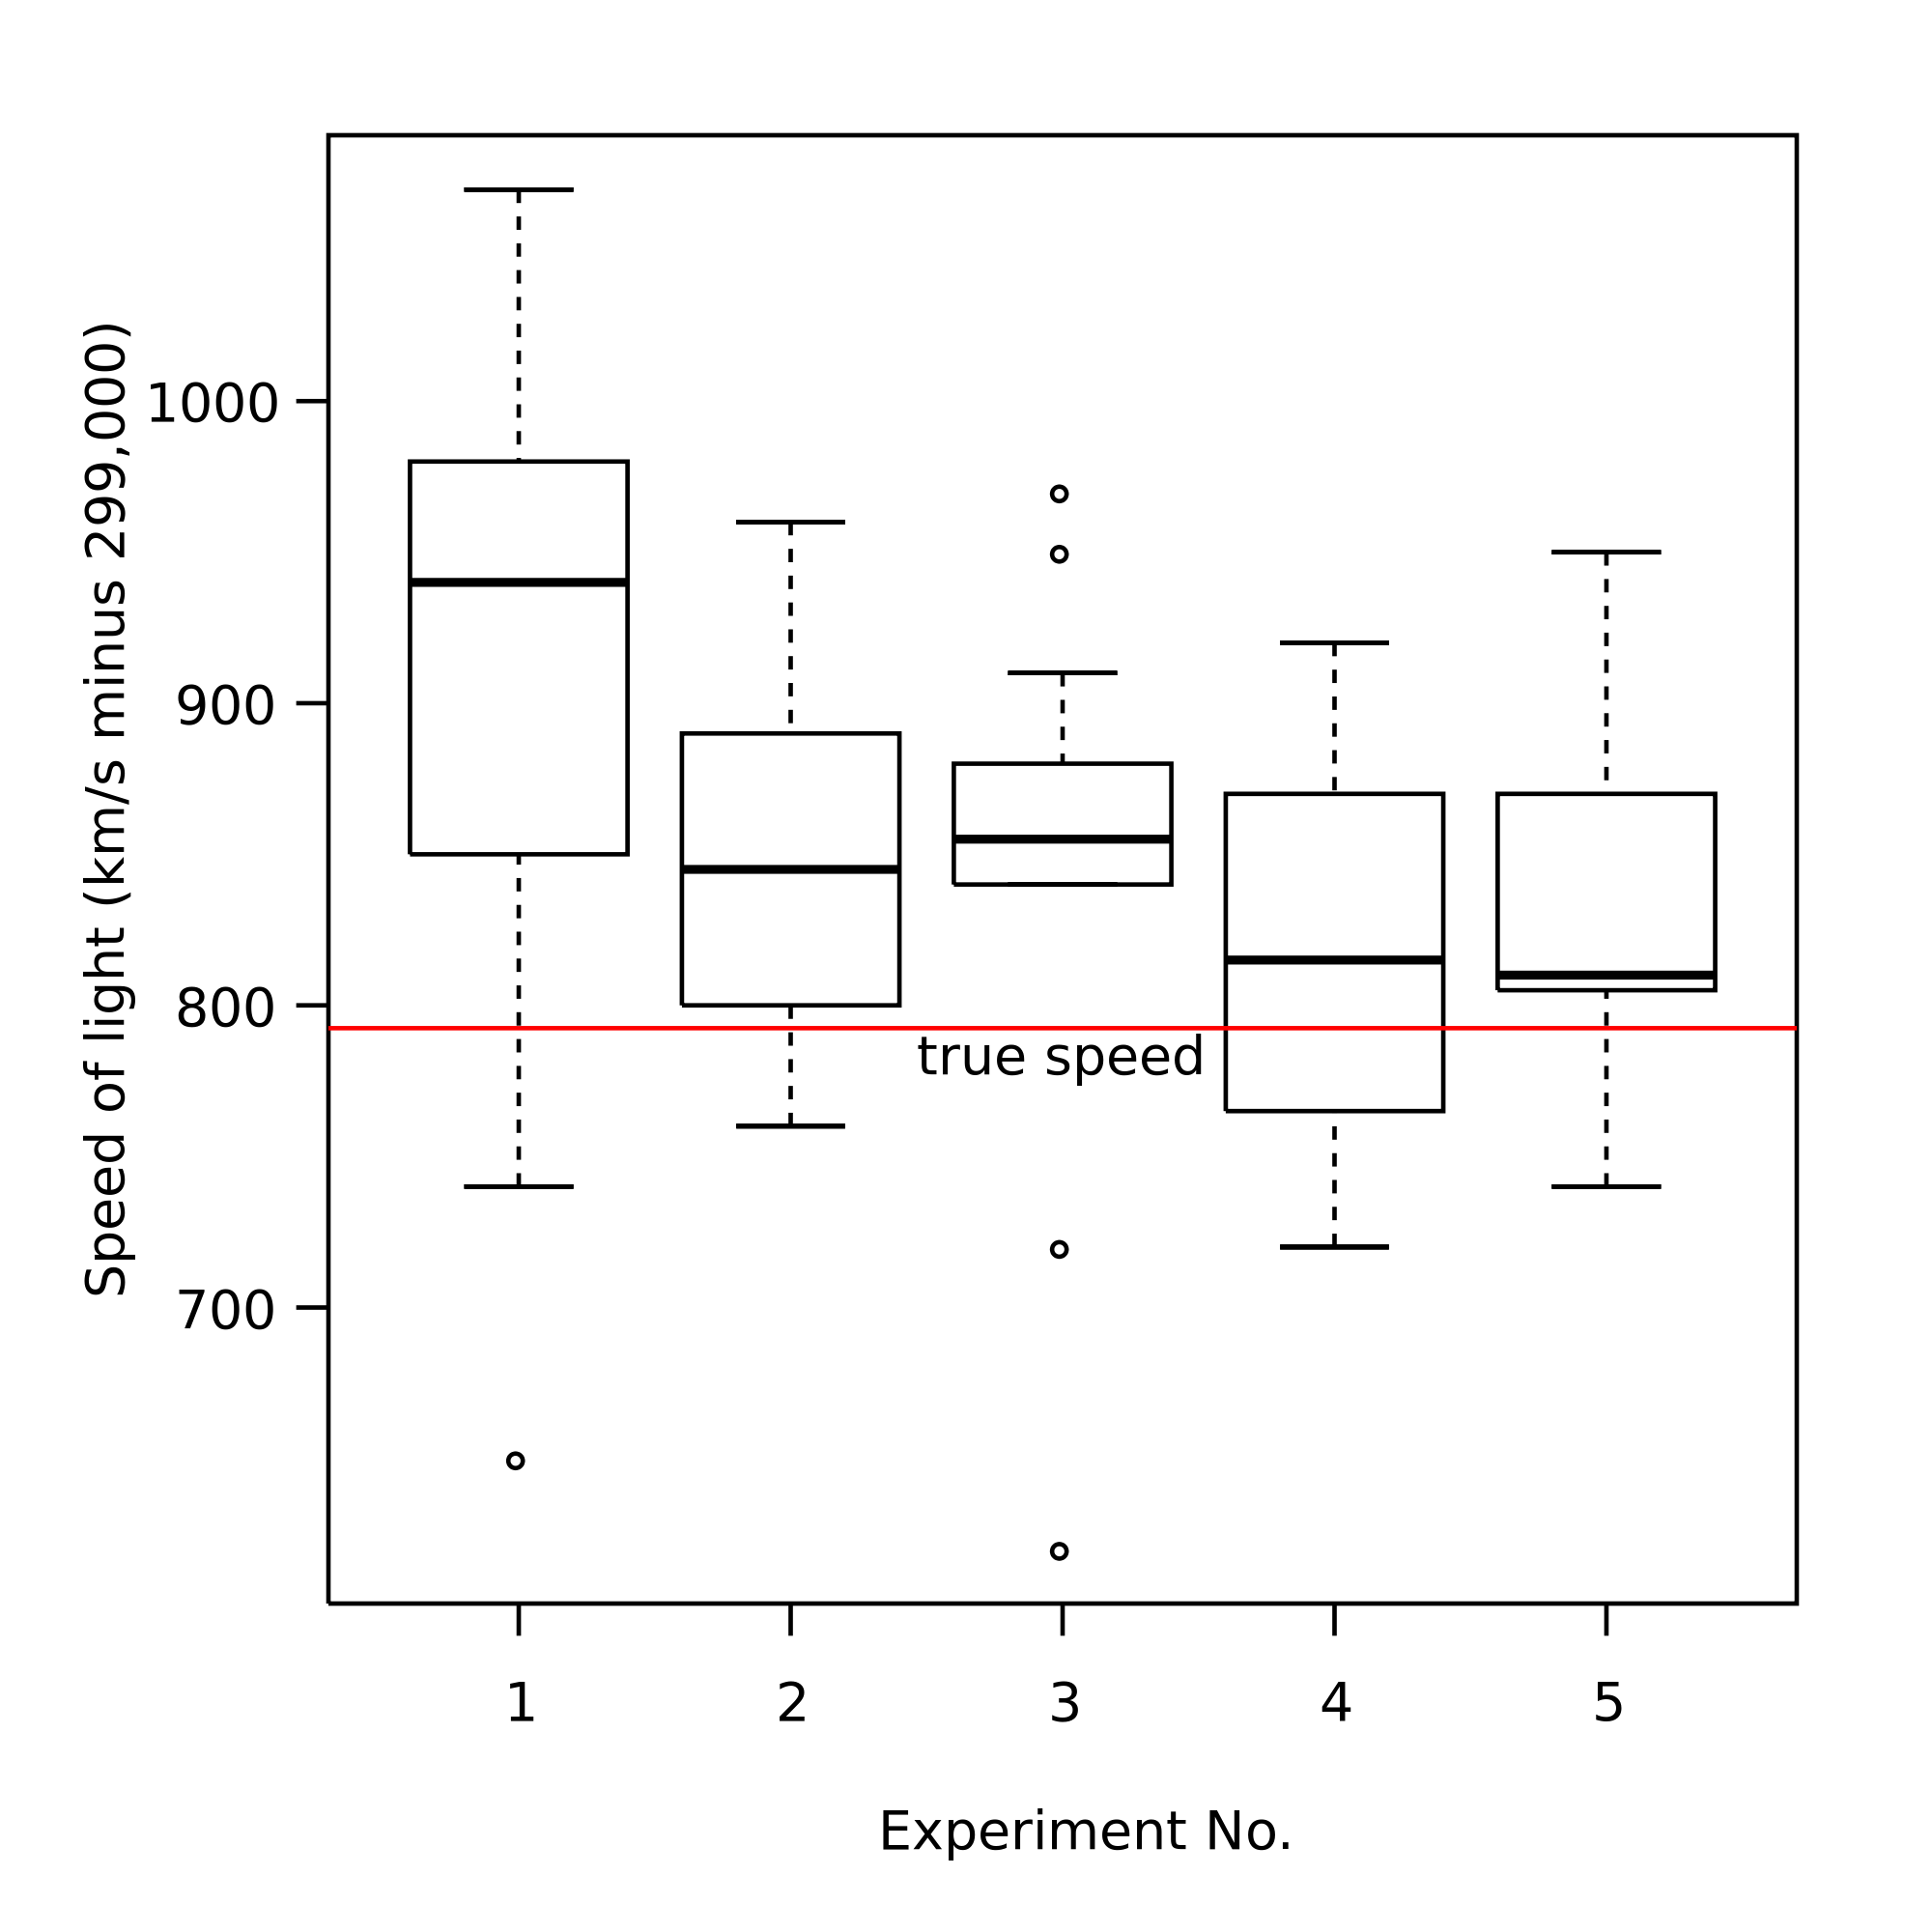
\includegraphics[width=.7\textwidth]{Intro/boxplot}

%       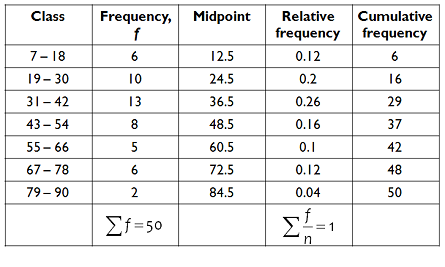
\includegraphics[width=.9\textwidth]{Intro/table}
% %[height=.5\textheight]
%       \end{center}
%     \end{column}
%   \end{columns}
% \end{frame}

% \begin{frame}{Trailer do curso}
% Vamos fazer um pequeno experimento didático

%   \begin{block}{Dados necessários}
%     \begin{itemize}
%     \item Sexo
%     \item Altura (cm)
%     \item Tamanho do sapato
%     \end{itemize}
%   \end{block}
% \end{frame}

\end{document}
